\documentclass[a4paper, 11pt]{article}
\usepackage{lipsum,url} 
\usepackage{fullpage} 
\usepackage{color}
\usepackage{algorithm,algorithmic}
\usepackage{graphicx}
\usepackage{amsmath}
\usepackage{comment}

% ----- math theorem ----- %
\usepackage{amsthm}
\newtheorem{theorem}{Theorem}
\newtheorem{claim}{Claim}
\newtheorem{remark}[theorem]{Remark}
\newtheorem{lemma}[theorem]{Lemma}
\newtheorem{proposition}[theorem]{Proposition}
\newtheorem{corollary}[theorem]{Corollary}
\newtheorem{definition}{Definition}
\newtheorem{exmp}{Example}[section]

\usepackage{amssymb}

\setlength\parindent{0pt}
\setlength{\parskip}{10pt}

\begin{document}

\begin{center}
\Large  CS4013/5013 Assignment 2\\[1em]
\large Fall 2025\\[1em] 
\end{center}

\vspace{20pt}

Due Date: Oct 3, 2025. 

\textit{Note: Written tasks will be posted 
on Canvas. Below is the description of 
programming tasks.}  




In this assignment, we will implement and apply 
search techniques to estimate some correlation in data.  
In the following, we will first describe the data, 
then formalize the estimation problem, and finally 
approach it from a search perspective. Assignment tasks 
are detailed at the end. 

\underline{1. A Credit Card Application Data Set}

We have a data set `CreditCard.csv' which contains 
the profile of 340 credit card applicants and their 
application results. Figure \ref{fig:hw2} is a 
screenshot of the data set, where each row contains 
the information of one applicant and the columns are attributes with the following interpretations. 

-- CreditApprove: `1' means application 
approved, `0' means denied. (Figure \ref{fig:hw2}
only shows `1'.)

-- Gender: `M' means male, `F' means female. 
You should encode `M' to 1 and `F' to 0. 

-- CarOwner: `Y' means yes, `N' means no. 
You should encode `Y' to 1 and `N' to 0. 

-- PropertyOwner: `Y' mean yes, `N' means no. 
You should encode `Y' to 1 and `N' to 0. 

-- \#Children: number of children. 

-- WorkPhone: `1' means the applicant has a 
work phone, `0' means otherwise. 

-- Email: `1' means the applicant has an 
email ID, `0' means otherwise. 

Note our data set is a subset of the public Credit Card data 
set\footnote{\url{https://www.kaggle.com/datasets/rohitudageri/credit-card-details}}. 

\begin{figure}[t!]
    \centering
    % \includegraphics[width=\linewidth]{figure/hw2_dataset.PNG}
    \caption{}
    \label{fig:hw2}
\end{figure}

\vspace{5pt}
\underline{2. The Correlation Estimation Problem}

Let $x$ denote an applicant and $y$ 
be his/her application result. Suppose there 
is a linear relation between $x$'s attributes 
and $y$, and we aim to approximate it using 
the following function 
\begin{equation}
f(x) = w_1 \cdot x^{(1)} + w_2 \cdot x^{(2)} + 
w_3 \cdot x^{(3)} + w_4 \cdot x^{(4)} + w_5 \cdot 
x^{(5)} + w_6 \cdot x^{(6)}, 
\end{equation}
where $x^{(j)}$ is the $j_{th}$ 
attribute of $x$ in the above table i.e., $x^{(1)}$ 
is gender, ..., $x^{(6)}$ is email. To facilitate 
later discussion, let us write 
$w := [w^{(1)}, w^{(2)}, w^{(3)}, 
w^{(4)}, w^{(5)}, w^{(6)}]$. 

The $w_j$'s are unknown parameters of the 
function taking values in $\{-1, +1\}$. 
Our goal is to find $w_j$'s that give the 
best approximation i.e., minimize 
the following approximation error 
\begin{equation}
er(w) := \frac{1}{n} \sum_{i=1}^n (f(x_i) - y_i)^2,   
\end{equation}
where $x_i$ is the $i_{th}$ applicant, 
$y_i$ is his/her application result 
and $n$ is the number of applicants in 
the data set. In our problem, $n = 340$. 

Problem $\min_{w} er(w)$ would be easier to solve 
if $w_j$'s are continuous (e.g., by taking 
derivative of $er(w)$). 
But we have assumed $w_j \in \{-1, +1\}$ 
for better interpretability of the estimated 
relation (which simply tells us which attributes are useful 
but not the degree of their usefulness). 
This makes $\min_{w} er(w)$ an integer programming 
problem that is harder to solve.  

\vspace{5pt}
\underline{3. Approach Estimation from a Search Perspective}

We can approach $\min_{w} er(w)$ from a `search' perspective. 
First, understand that there are many possible $w$'s 
which may or may not minimize $er(w)$. Below are three examples

-- $w = [1, 1, -1, -1, 1, -1]$

-- $w = [-1, -1, -1, -1, 1, 1]$

-- $w = [1, 1, 1, 1, 1, 1]$

Now, we can apply search techniques to find an 
optimal $w$, and optimality is measured by $er(w)$. 
Below is an example search process. 

Step 1. Initialize $w = [-1,-1,-1,-1,-1,-1]$ 
is an initial solution (randomly picked) 

Step 2. Pick the next solution e.g., $w' = [1, 1, 1, 1, 1, 1]$. If $er(w') < er(w)$, update $w = w'$.

Step 3. Repeat step 2 until convergence. 

Note different search techniques pick the next $w$ with different strategies e.g., local search picks $w'$ that is adjacent to $w$ (with a proper definition of adjacency) 
and evolutionary search generates $w'$ with proper probability. 

Also note the above example process only picks and 
examines one $w'$ at a time, while some search techniques 
may pick and examine a bag of $w'$'s at a time (and 
update $w$ to the best). 

\newpage 

\textbf{\large Programming Tasks}


\underline{Task 1}. Implement hill climbing local search 
algorithm and apply it to find the $w$ that 
(aims to) minimize $er(w)$. 
Recall that in each round of local search, we examine 
all solutions adjacent to the current solution and 
identify the best one. We define adjacency as follows: 

\textit{Two solutions $w$ and $w'$ are adjacent if they 
differ by exactly one element e.g., $w = [1,1,1,1,1,1]$ 
and $w' = [-1,1,1,1,1,1]$ are adjacent, so are 
$w = [-1,-1,1,1,1,1]$ and $w' = [-1,-1,1,1,-1,1]$.} 


After implementation, you need to present two results below. 

-- In Figure \ref{fig:hw2t1}, plot a curve of 
$er(w)$ versus the round of search. 
The x-axis of this figure is the round of search and the y-axis of this figure is $er(w)$. Your figure should include 
enough rounds so we can see $er(w)$ converges. 

\begin{figure}[h!]
    \centering
    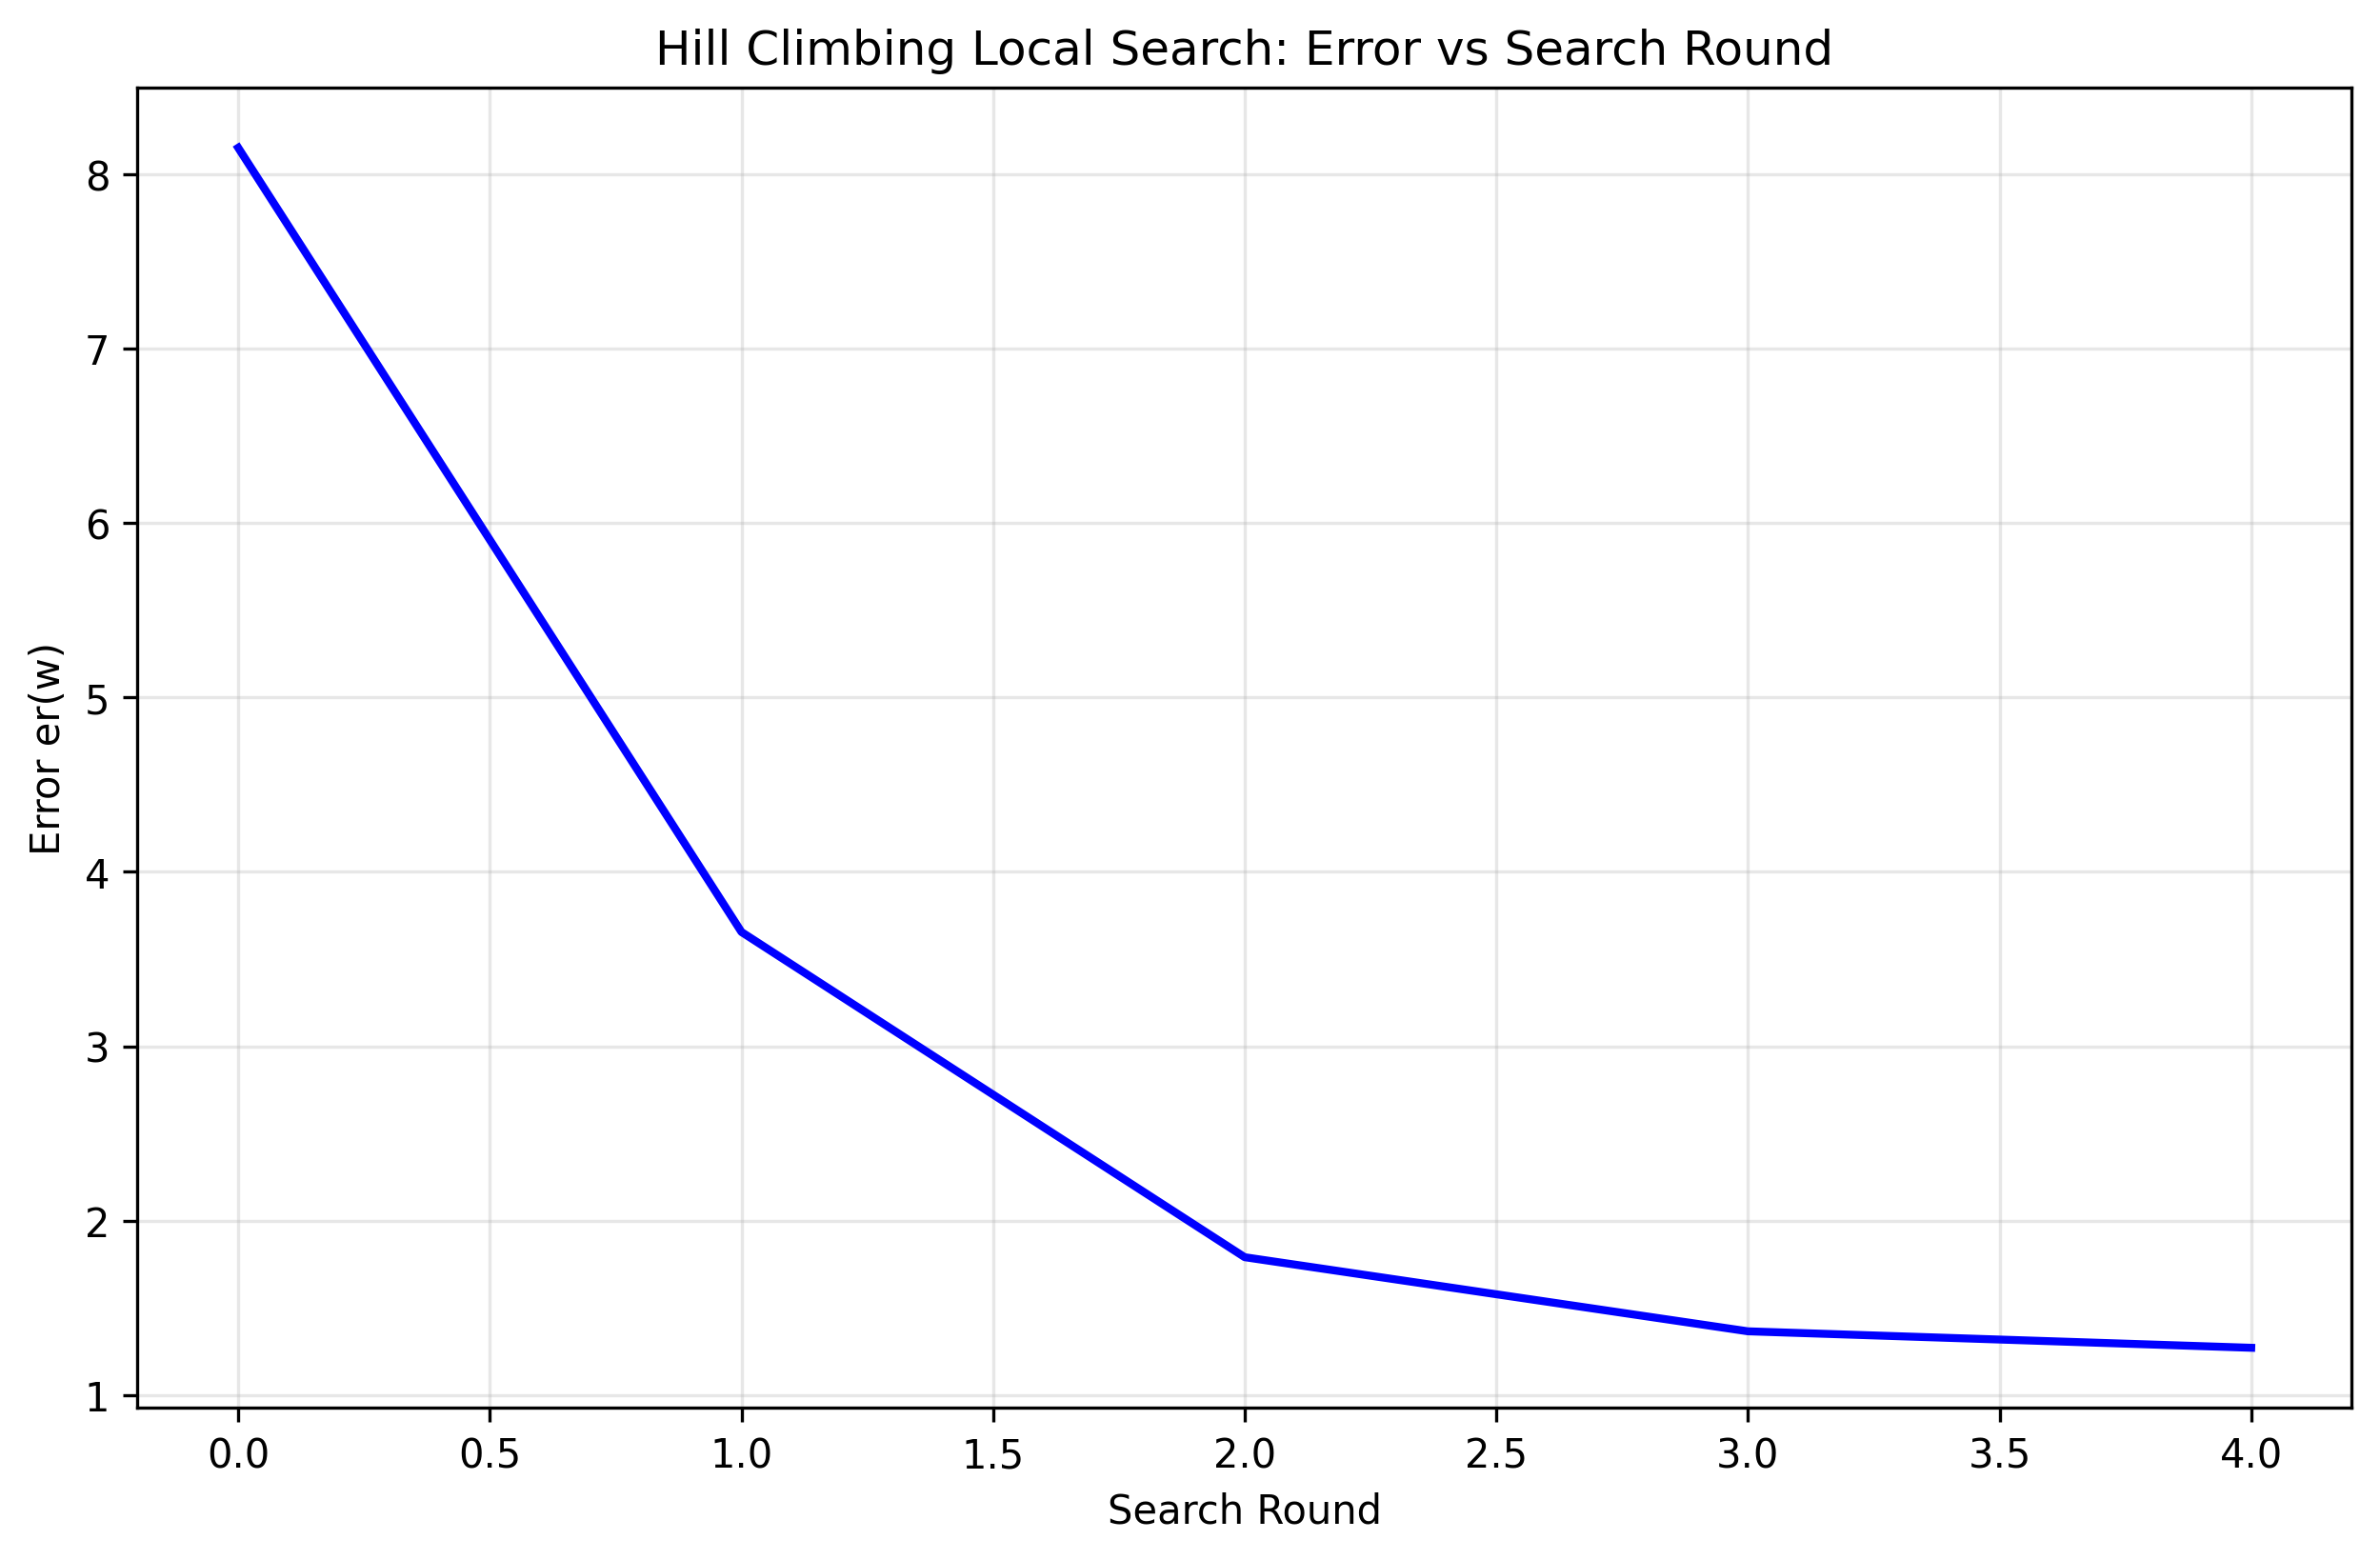
\includegraphics[width=0.8\linewidth]{../../local_search_error.png}
    \caption{Error vs search round for hill climbing local search algorithm}
    \label{fig:hw2t1}
\end{figure}

-- Present the optimal $w$ and $er(w)$ returned by your search algorithm below. 
\begin{equation}
\label{eq:t1w}
w = [1, -1, 1, -1, 1, 1]
\end{equation}
\begin{equation}
\label{eq:t1er}
er(w) = 1.2713864306784661
\end{equation}

\vspace{10pt}

\underline{Task 2}. Implement the genetic algorithm 
and apply it to find $w$ that (aims to) minimize 
$er(w)$. Treat each $w$ as a chromosome (note it 
is a binary string) and treat $e^{-er(w)}$ as  
fitness function. You can configure the genetic algorithm 
by yourself. But here are some suggestions

-- Do not set the population size too large. 
Keep in mind $w$ contains only six binary 
variables, which means there are at most  
$2^6 = 64$ different $w$'s. 

-- Set the number of parents that come together to form
offspring to 2. 

-- When you select chromosomes to be the parents 
of the next generation, 
select them based on probabilities proportional 
to their fitness values. You can generate probabilities 
by normalization e.g., suppose there are three candidate 
chromosomes in with fitness values $0.1, 2, 0.8$, then 
their selection probabilities can be computed as  
\begin{equation}
0.1 \rightarrow \frac{0.1}{0.1+2+0.8} = 0.034    
\end{equation}
\begin{equation}
2 \rightarrow \frac{2}{0.1+2+0.8} = 0.689  
\end{equation}
\begin{equation}
0.8 \rightarrow 1 - 0.034 - 0.689 = 0.277
\end{equation}

-- Fix the crossover point to the middle of 
$w$ i.e., the first three elements of one $w$ 
gets to be recombined with the last elements 
of another $w'$. 

-- Set the mutation rate by yourself. Try small 
values first. 

After implementation, you need to present two results 
(based on your chosen configuration) below. 

-- In Figure \ref{fig:hw2t2}, plot a curve of 
$er(w)$ versus generation. 
The x-axis of this figure is the round of 
generation and the y-axis of this figure is $er(w)$. Your figure should include enough generations so we 
can see $er(w)$ converges. 

\begin{figure}[h!]
    \centering
    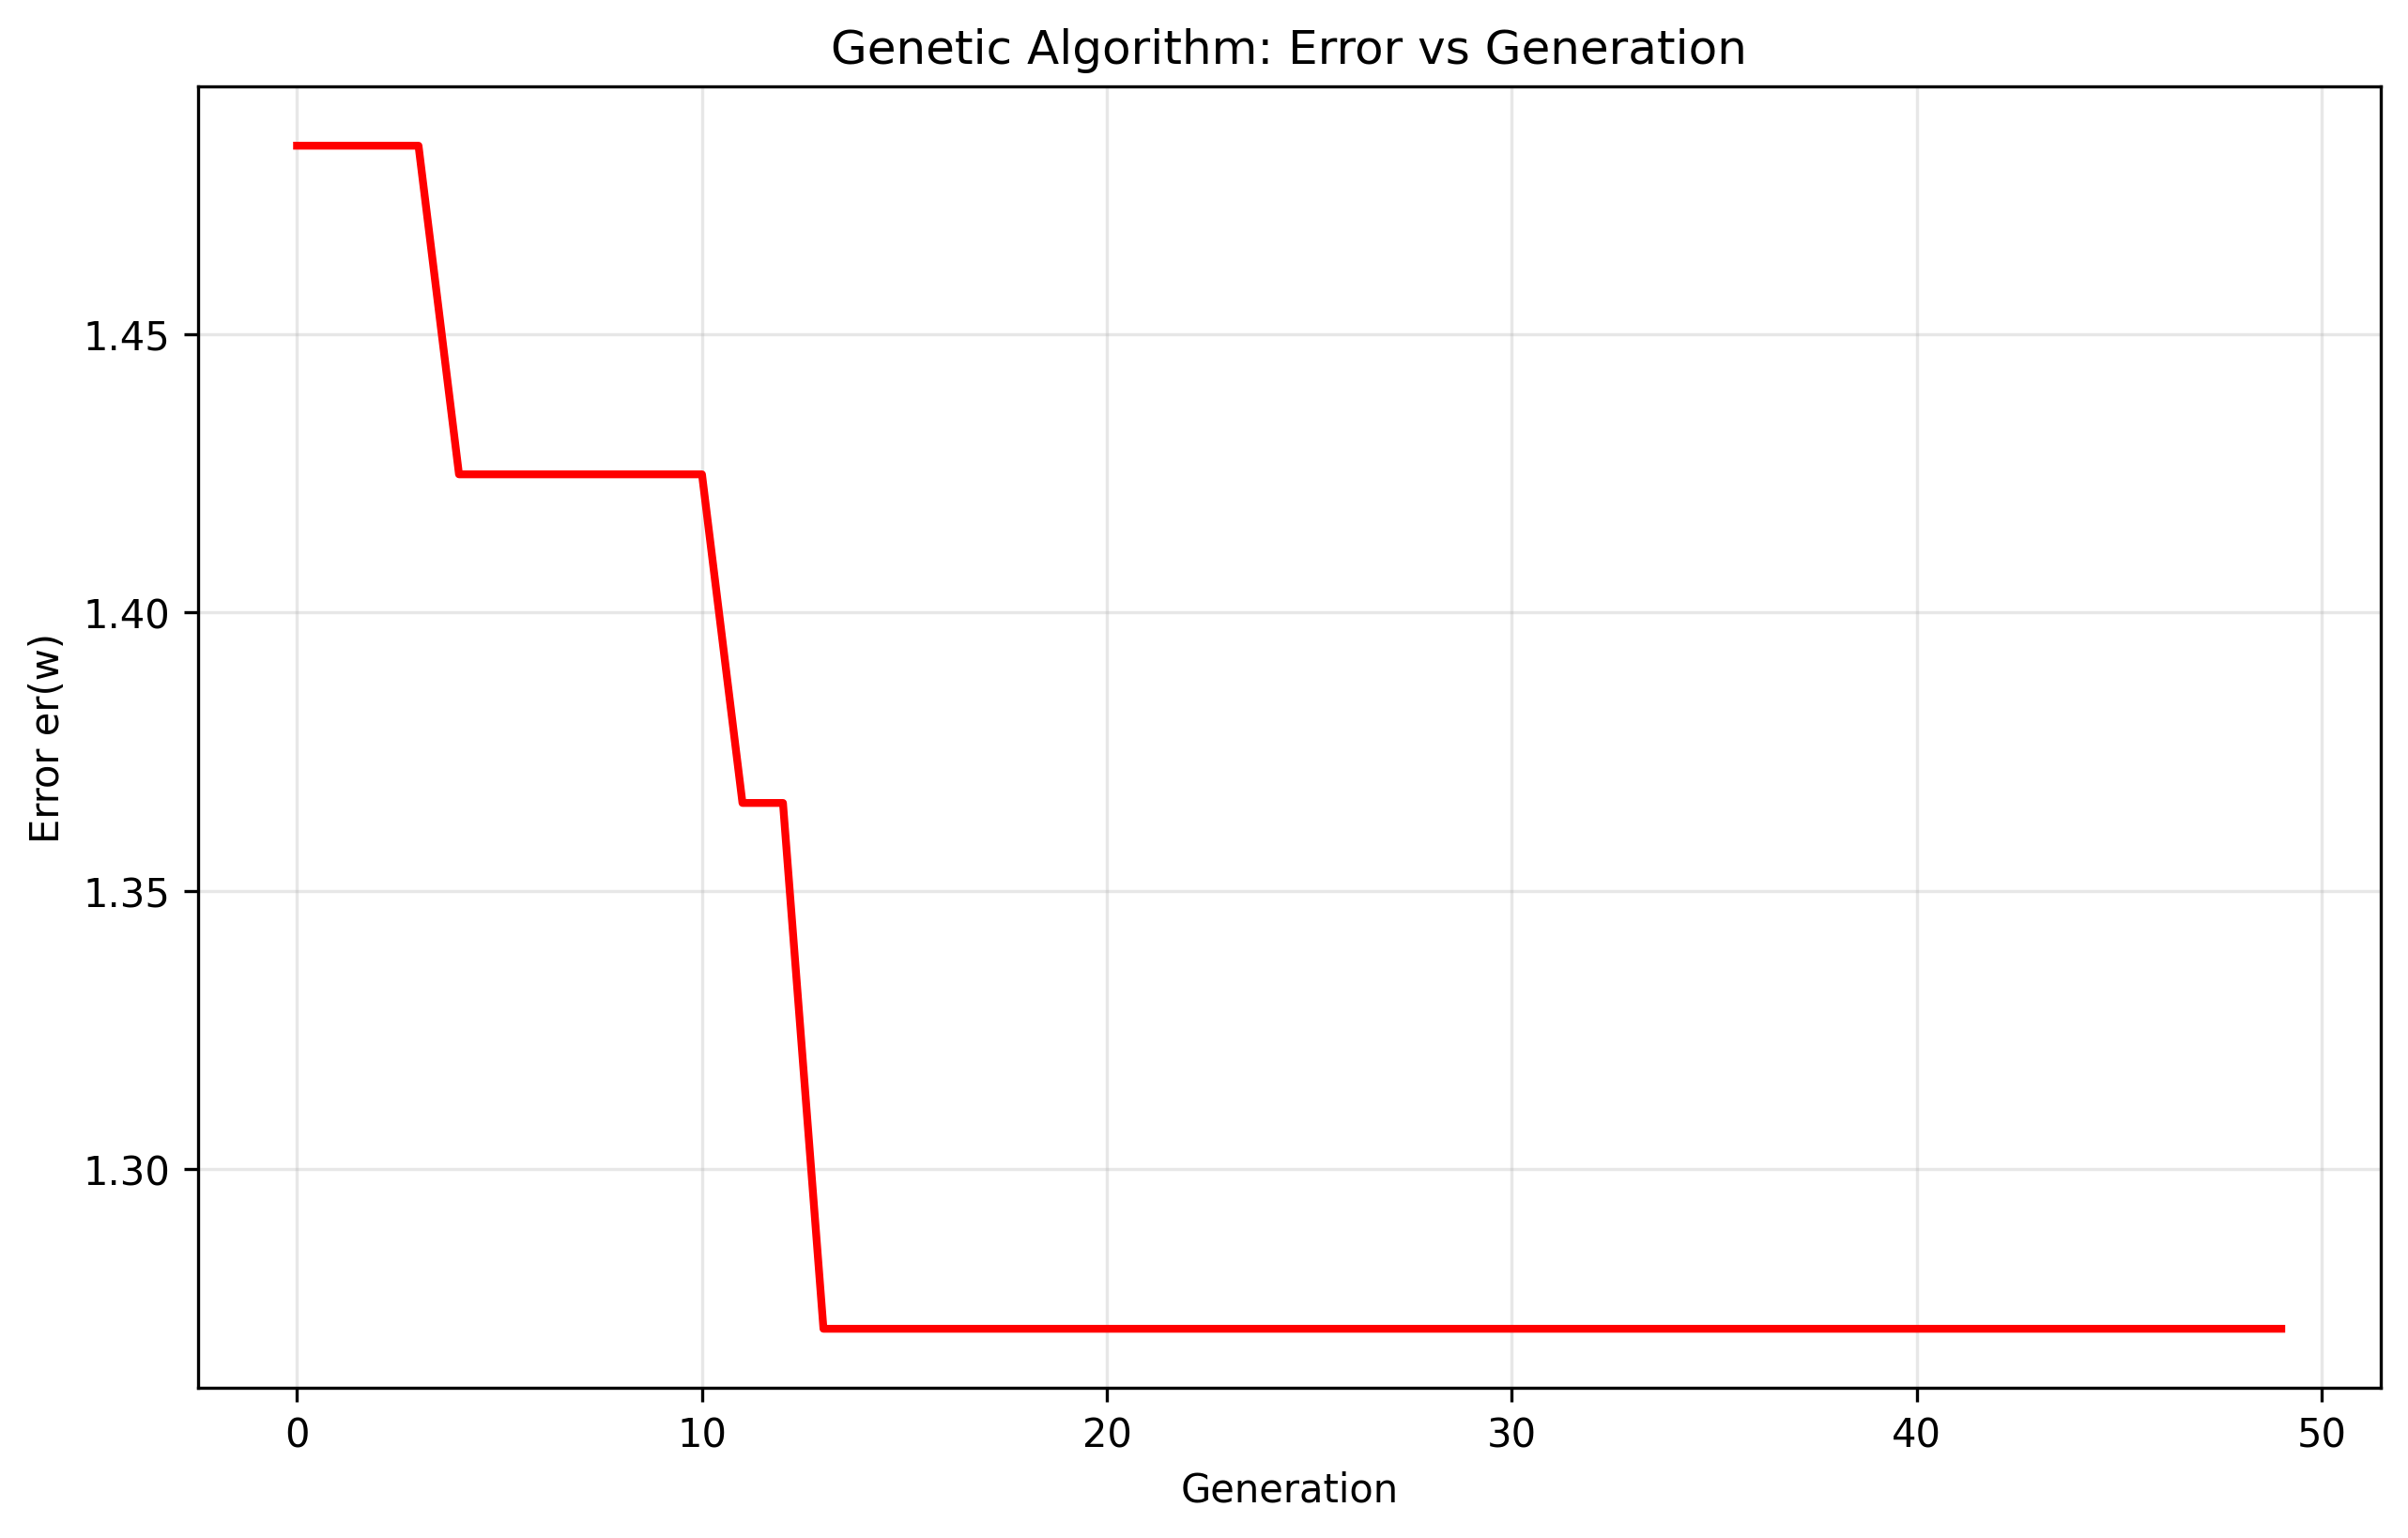
\includegraphics[width=0.8\linewidth]{../../genetic_algorithm_error.png}
    \caption{Error vs generation for genetic algorithm}
    \label{fig:hw2t2}
\end{figure}

-- Present the optimal $w$ and $er(w)$ returned by your search algorithm below. 
\begin{equation}
\label{eq:t2w}
w = [1, -1, 1, -1, 1, 1]
\end{equation}
\begin{equation}
\label{eq:t2er}
er(w) = 1.2713864306784661
\end{equation}

\underline{Submissions Instructions}

You should generate 6 results for the programming tasks, including 

(1) a figure of $er(w)$ versus search round for local search, 
placed in Figure \ref{fig:hw2t1}.

(2) optimal $w$ and $er(w)$ returned by local search, 
placed in equations (\ref{eq:t1w}) and (\ref{eq:t1er})

(3) a figure of $er(w)$ versus generation for genetic algorithm, place in Figure \ref{fig:hw2t2} 

(4) optimal $w$ and $er(w)$ returned by genetic algorithm, 
placed in equations (\ref{eq:t2w}) and (\ref{eq:t2er})

(5) a Python code named `hw2\_local.py' that generates 
the figure in (1) 

(6) a Python code named `hw2\_genetic.py' that generates the figure in (2)

You should place results (1)(2)(3)(4) in a pdf 
file named `hw2.pdf' and upload it to Canvas 
through the submission page for hw2. You also need 
to upload hw2\_local.py and hw2\_genetic.py. 

A latex template `hw2\_Latex.txt' will be provided. 
\end{document}